\documentclass[11pt]{scrartcl}
\usepackage{fullpage}
\usepackage{placeins}


\usepackage{listings} % Coding Syntax coloring
\usepackage{color}
\usepackage{textcomp}
\definecolor{listinggray}{gray}{0.9}
\definecolor{lbcolor}{rgb}{0.9,0.9,0.9}

\usepackage{amsmath}
\usepackage{textcomp}

\lstset{
     backgroundcolor=\color{lbcolor},
     tabsize=4,
     rulecolor=,
     language=matlab,
        basicstyle=\scriptsize,
        upquote=true,
        aboveskip={1.5\baselineskip},
        columns=fixed,
        showstringspaces=false,
        extendedchars=true,
        breaklines=true,
        prebreak = \raisebox{0ex}[0ex][0ex]{\ensuremath{\hookleftarrow}},
        frame=single,
        showtabs=false,
        showspaces=false,
        showstringspaces=false,
        identifierstyle=\ttfamily,
        keywordstyle=\color[rgb]{0,0,1},
        commentstyle=\color[rgb]{0.133,0.545,0.133},
        stringstyle=\color[rgb]{0.627,0.126,0.941},
}
\usepackage{fancyhdr,graphicx,lastpage}% http://ctan.org/pkg/{fancyhdr,graphicx,lastpage}
\fancypagestyle{plain}{
  \fancyhf{}% Clear header/footer
  \fancyhead[R]{
\includegraphics[scale=0.5]{logo.png}}% Right header
  \fancyhead[L]{\textbf{School of Electronic and Electrical Engineering}}
  %\fancyfoot[L]{Name Firstname - v1.0 \\  Date}% Left footer
  \fancyfoot[R]{\thepage\  / \pageref{LastPage}}% Right footer
}
\pagestyle{plain}% Set page style to plain.


\begin{document}
\title{ELEC2430 Matlab Assignment 1}
\subtitle{ Amplitude Modulation System and Spectrum Analysis}
\author{Yingjie Luan}
\maketitle

\tableofcontents

\section{Laboratory works}
\subsection{performance analysis }
Below is the table of SNR(Signal to Noise ratio) and BER(bit error rate),

\FloatBarrier
\resizebox{\textwidth}{!}{
\begin{tabular}{|l|l|l|l|l|l|l|l|l|l|l|l|}
\hline
1&2&3&4&5&6&7&8&9&10&11&12\\\hline
0.017129&0.008987&0.0040556&0.0015898&0.0004967&0.0001243&2.01e-05&2.2e-06&0&0&0&0\\\hline
\end{tabular}}
\FloatBarrier


\begin{minipage}[t]{\linewidth}
%\label{fig:main}

{
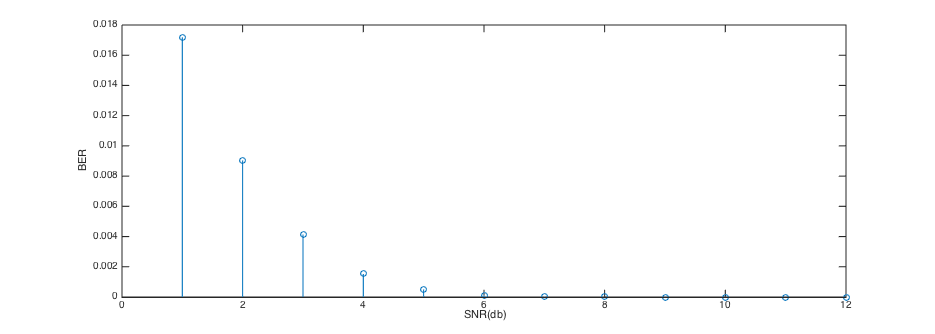
\includegraphics[scale = 0.5]{per.png}
\captionof{figure}{This is the SNR to BER ratio, the BER is decreasing as the noise getting decreased}
}
\end{minipage}
\medskip

Overall, there are 1 million data points for each experiment and it was conducted for 10 times to get the average result.
\subsection{time domain analysis }

\subsubsection{Binary signal}
\begin{minipage}[t]{\linewidth}
%\label{fig:main}

{
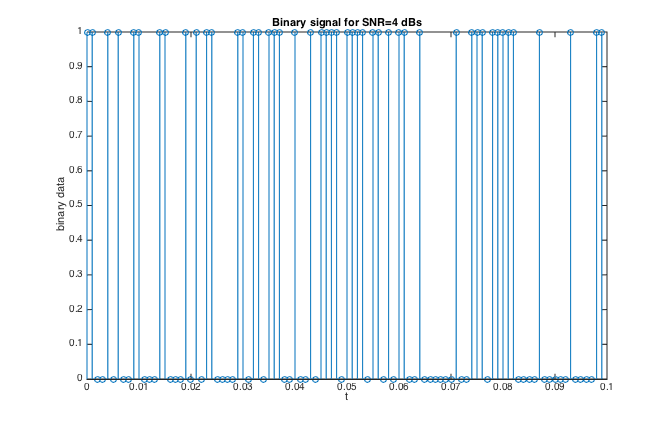
\includegraphics[scale = 0.6]{Binary_signal.png}
\captionof{figure}{This is the plot of the first 100 bits of the binary signal.}
}
\end{minipage}
\medskip
\subsubsection{Sampled signal}
\begin{minipage}[t]{\linewidth}
{
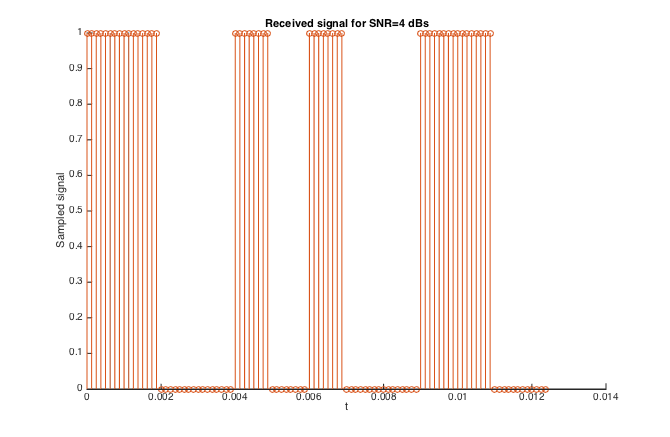
\includegraphics[scale = 0.6]{Sampled_signal.png}
\captionof{figure}{This is the plot of the first 100 bits of the sampled signal.}
}
\end{minipage}
\medskip

\subsubsection{Modulated Signal}
\label{sec:before}
\begin{minipage}[t]{\linewidth}
{
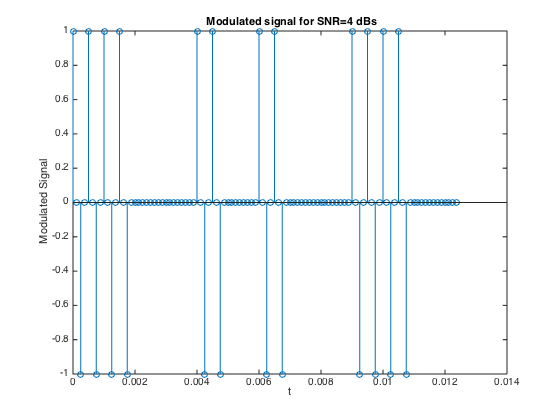
\includegraphics[scale = 0.6]{Modulated_signal.png}
\captionof{figure}{This is the plot of the first 100 bits of the modulated signal.}
}
\end{minipage}
\medskip

\subsubsection{Received signal}
\label{sec:after}
\begin{minipage}[t]{\linewidth}
{
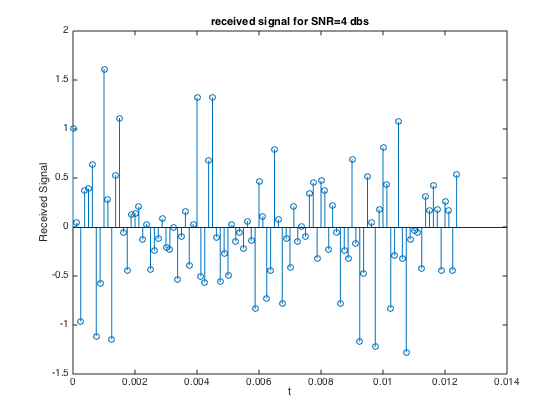
\includegraphics[scale = 0.6]{received_signal.png}
\captionof{figure}{This is the plot of the first 100 bits of the received signal.}
}
\end{minipage}
\medskip

\subsubsection{Filtered signal}
\begin{minipage}[t]{\linewidth}
{
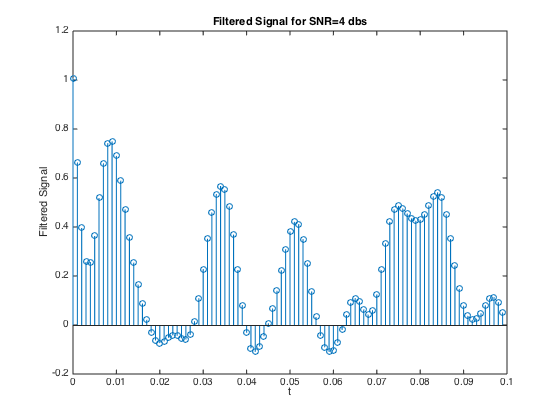
\includegraphics[scale = 0.6]{filtered_signal.png}
\captionof{figure}{This is the plot of the first 100 bits of the filtered signal.}
}
\end{minipage}
\medskip


\subsection{frequency domain analysis }
Below is the required plot, in total, the number of data point is 1 million.
\subsubsection{Sampled signal}
\begin{minipage}[t]{\linewidth}
{
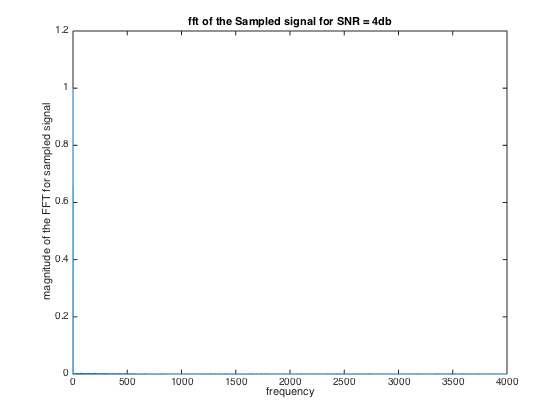
\includegraphics[scale = 0.6]{sampled_signal_fft.png}
\captionof{figure}{This is the plot of the  FFT of the sampled signal.}
}
\end{minipage}
\medskip

\subsubsection{Modulated signal}
\begin{minipage}[t]{\linewidth}
{
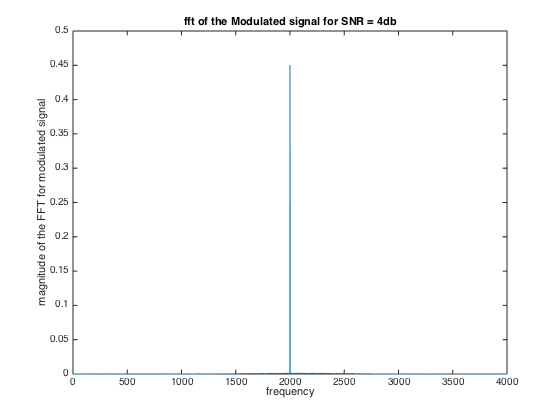
\includegraphics[scale = 0.6]{modulated_signal_fft.png}
\captionof{figure}{This is the plot of the FFT of the sampled signal.}
}
\end{minipage}
\medskip

\subsubsection{Received signal}
\begin{minipage}[t]{\linewidth}
{
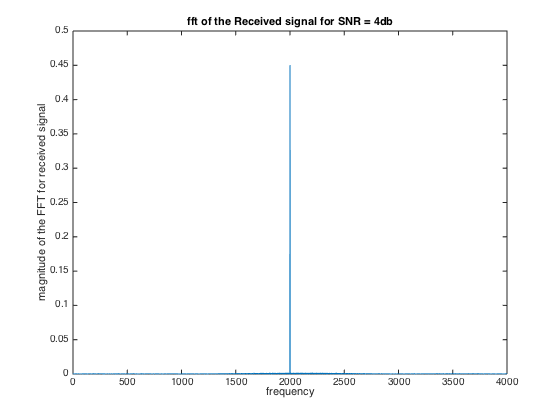
\includegraphics[scale = 0.6]{received_signal_fft.png}
\captionof{figure}{This is the plot of the FFT of the received signal.}
}
\end{minipage}
\medskip

\subsubsection{Filtered signal}
\begin{minipage}[t]{\linewidth}
{
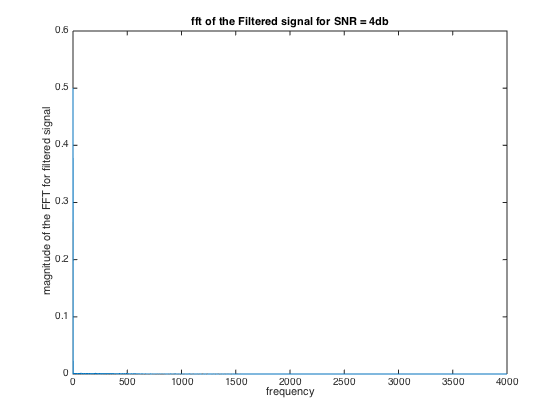
\includegraphics[scale = 0.6]{filtered_signal_fft.png}
\captionof{figure}{This is the plot of the FFT of the filtered signal.}
}
\end{minipage}
\medskip

\section{Result Analysis}

\subsection{Question 1}
\subsubsection{What is the effect of the noise?}
Noise simulated the uncertainty in the real environment. Section \ref{sec:before}'s image is the signal before going through noise channel and section \ref{sec:after}'s image is the same signal after it has gone through the noise channel. It has a repercussion on the transmitted signal in time otherwise our BER would all be 0.

\subsubsection{What happened when SNR increases}

When SNR increases(Which means noise attenuates) BER decrease. 

\subsubsection{What is the reason behind this performance}
Below is a series of image to demonstrate this effect:

\begin{minipage}[t]{\linewidth}
{
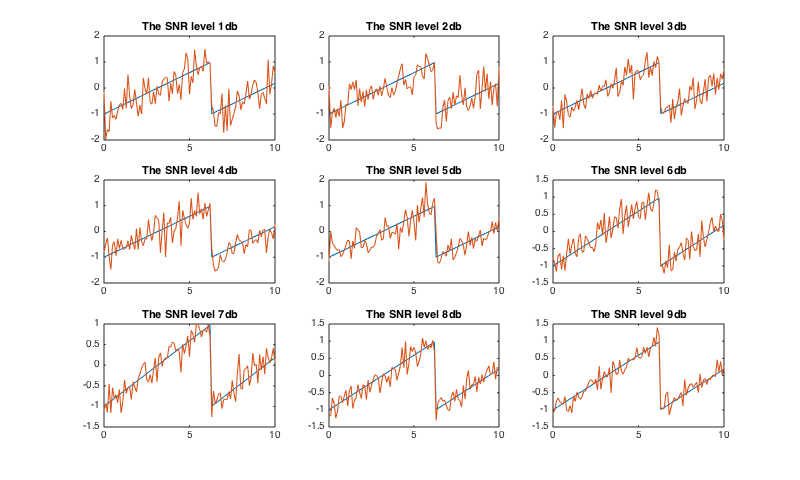
\includegraphics[scale = 0.6]{demo_snr.png}
\captionof{figure}{As SNR increases the noise get attenuated.}
}
\end{minipage}
\medskip

Because noise get attenuated we get a more accurate response which helps us to decease the BER.

\subsection{Question 2}

The effect of the filter is to help us to remove the high frequency component within the demodulated signal, as we can see from the figure below :

\begin{center}
\begin{minipage}[t]{\linewidth}
%\label{fig:main}

{
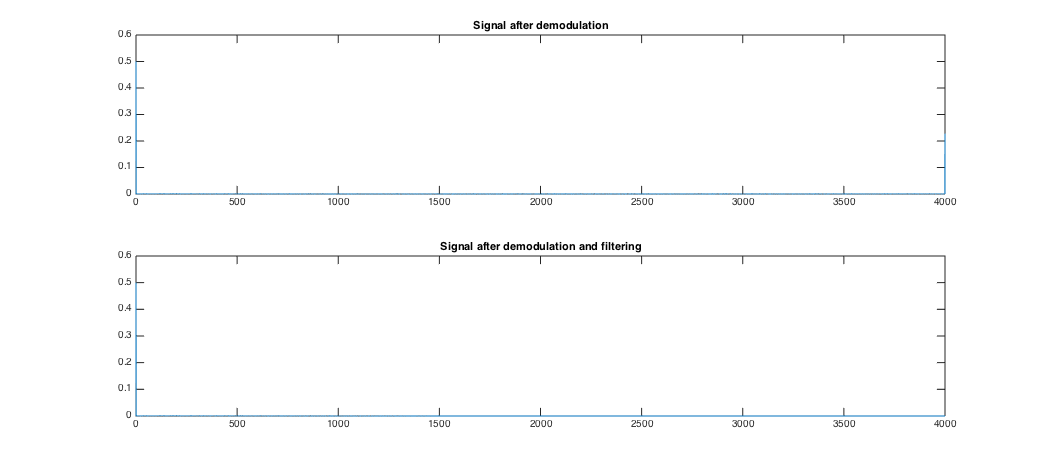
\includegraphics[scale = 0.5]{butter.png}
\captionof{figure}{This is the comparison of the signal before and after the filtering.}
}
\end{minipage}
\medskip
\end{center}
  
\subsection{Appendix}
\subsubsection{Matlab code for doing the simulation}
\begin{lstlisting}[language=Matlab]
function ber =  main(snr)
% the code is to get all the related data from a single execution
    N = 1000000;
    data_rate = 1000;
    % creating N bits, the bit rate is 1000bps(1000 bits per second)

    data = randint(N,1);
    Fs = 8000; % sampling frequency
    data_t = 0:1/data_rate:(N-1)/data_rate;
    samplesPerBit  = Fs/data_rate;

%     k=1;
%     for i = 1:N
%         for j = 1:samplesPerBit  % these loops create the
%             y(k) = data(i);      % bit stream: y is 8000hz(8000 samples per second), data is 1000 samples per second
%             k=k+1;
%         end 
%     end  
    y=repmat(data,1,samplesPerBit)';
    y = y(:)';


    end_time = length(y)*(1/Fs);
    t = linspace(0,end_time,length(y));% the sampled time sequence : it is like the data_t
    fc = 2000;
    carrier = cos(2*pi*fc*t);
    % plot(carrier)

    modulated_signal = carrier.*y;

    % snr = 3; %3db
    noised_signal = awgn(modulated_signal,snr,'measured');

    demodulate_signal = noised_signal.*carrier;
    [b,a] = butter(5,fc/Fs);
    Filtered_signal = filtfilt(b,a,demodulate_signal);
% 
%     new_data = zeros(1,length(data));
    
%     for index = 1:samplesPerBit:length(y)
%         temp = Filtered_signal(index:index+samplesPerBit-1);
%         new_data(ceil(index/8)) = mean(temp) > 0.25;  %attundate by half
%     end
%     
    yy = reshape(Filtered_signal,samplesPerBit,[]);
    temp = mean(yy);
    new_data = temp > 0.25;
    
    ber = 1 - length(find(data==new_data'))/length(data);

\end{lstlisting}

\subsubsection{Matlab code for plotting FFT}

\begin{lstlisting}[language=Matlab]
function plot_fft(tk,Fs)

%Fs: sample rate
%tk: the signal in time sequence
% Plot the signal inthe 

    L = length(tk);
    NEET = 2^nextpow2(L);
    Y = fft(tk,NEET)/L;
    f = Fs/2*linspace(0,1,NEET/2+1);
    plot(f,2*abs(Y(1:NEET/2+1)));
\end{lstlisting}





\end{document}
